\subsection{Encoding}
\label{sec:encoders}

% figure pics/transformer.jpg

\begin{figure}[H]]
    \centering
    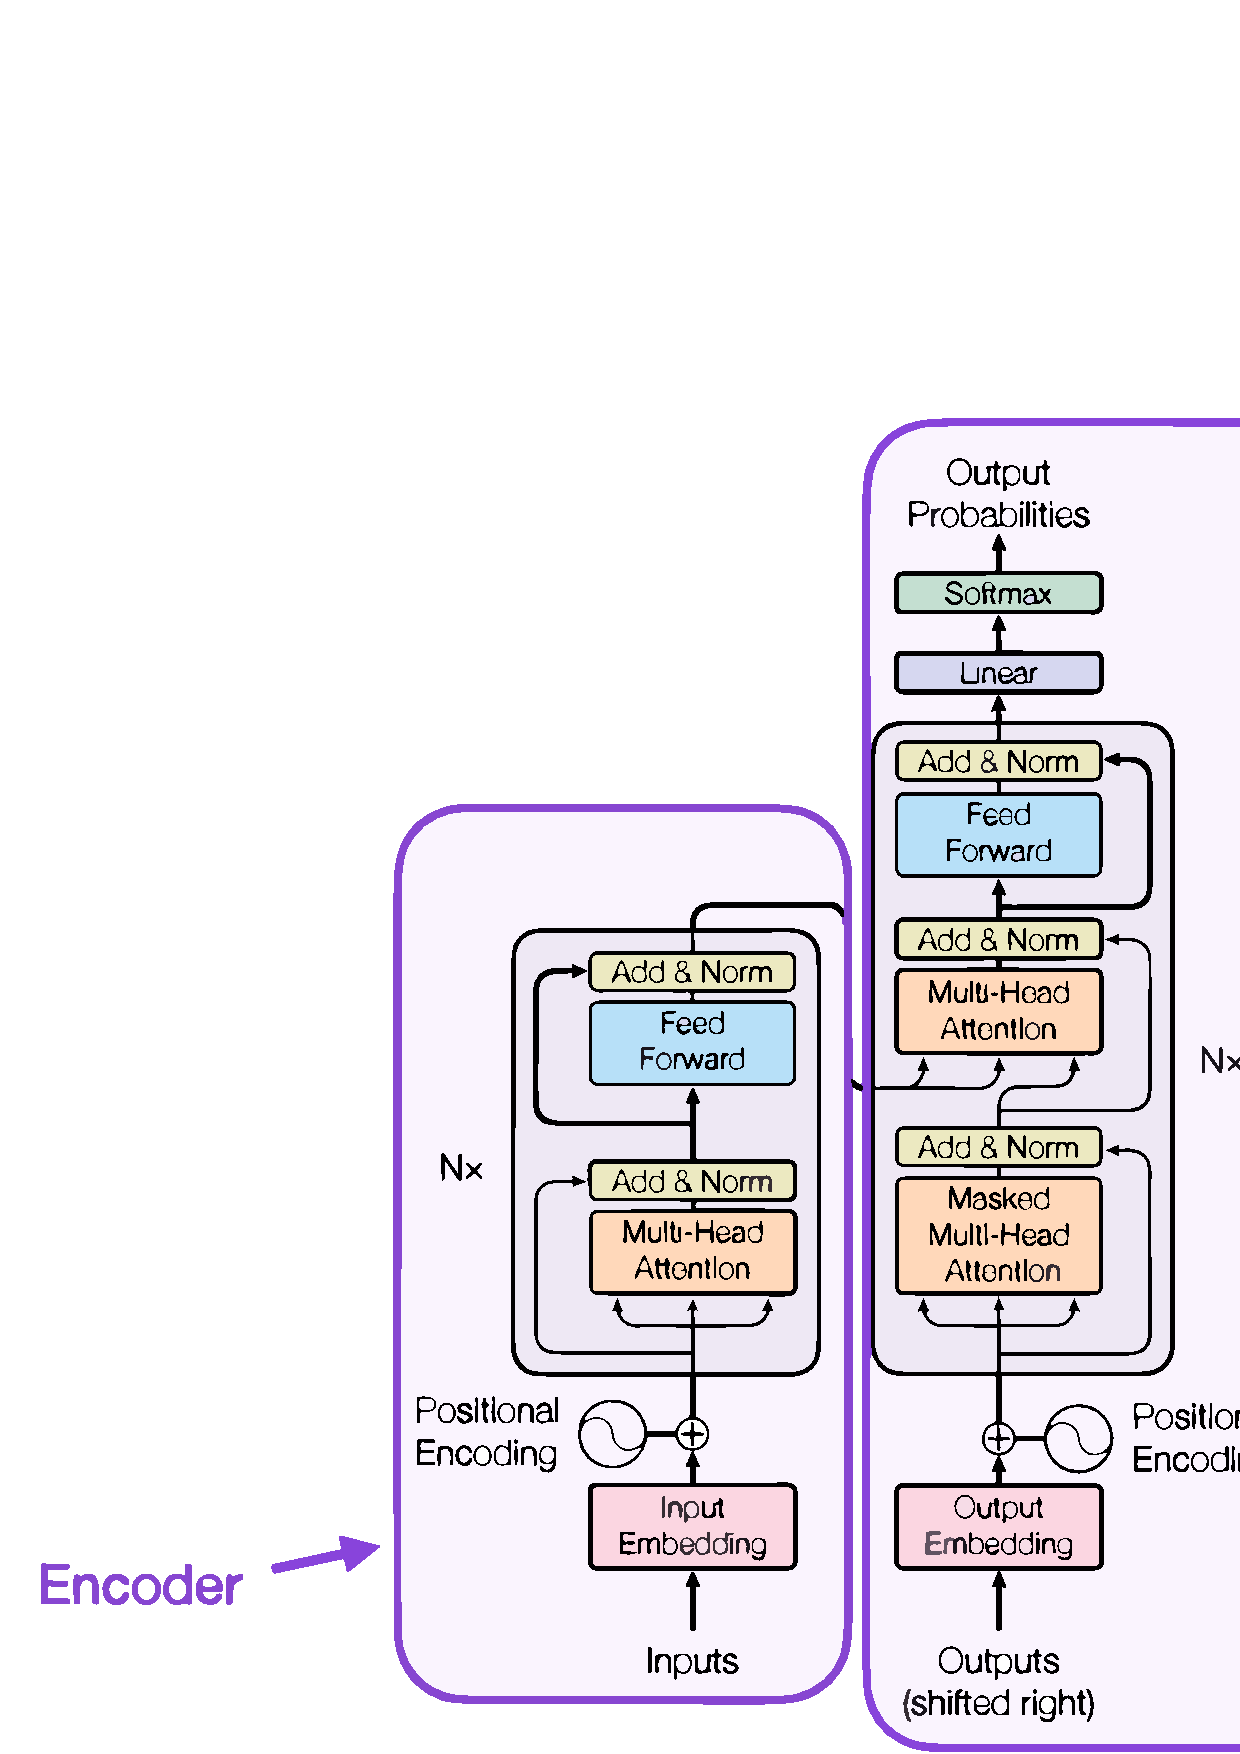
\includegraphics[width=0.8\linewidth]{pics/transformer.jpg}
    \caption{Transformer architecture featured in “Attention is all you need” \cite{https://doi.org/10.48550/arxiv.1706.03762}}
    \label{fig:transformer}
\end{figure}

Encoders\cite{kumar2022deep} are a crucial component in natural language processing tasks and consist of a multi-layered assembly of recurrent elements, such as Long Short-Term Memory (LSTM) units, Gated Recurrent Units (GRUs), or other similar structures. These recurrent elements work in tandem to process an input sequence, with each unit being responsible for handling a single element within the sequence, capturing the pertinent information for that specific element, and subsequently propagating this information forward to the next recurrent unit in the stack.

The primary function of an encoder is to systematically transform textual data into a suitable numerical or vector representation that retains the inherent relationships and dependencies among words, phrases, and sentences\cite{cho-etal-2014-learning}. This is achieved through a combination of techniques, such as tokenization, embedding, and the use of attention mechanisms, which together facilitate the encoding process.

Tokenization serves to break down the input text into smaller, manageable units, such as words or subwords, while embeddings assign a dense vector representation to each token, thus allowing machines to efficiently process and compare these tokens. Attention mechanisms, on the other hand, enable encoders to weigh the importance of different input elements and selectively focus on the most relevant parts of the input sequence when generating the final encoded representation.

By effectively converting the textual data into a machine-understandable format, encoders play a pivotal role in empowering machines to recognize intricate patterns, relationships, and contextual cues within the text. Consequently, this ability to accurately discern the context of sentences and phrases forms the foundation for a wide array of natural language processing tasks, ranging from machine translation and sentiment analysis to text summarization and question-answering systems.

Several approaches have been explored to address the challenges of representing the meaning of questions, capturing the structure of database schemas, and establishing connections between database content and questions in the text-to-SQL domain\cite{deng2022recent}. These methods play a crucial role in facilitating the understanding of the complex relationships between natural language questions and their corresponding SQL queries.

One of the main challenges in text-to-SQL research is effectively representing the meaning of questions. Various encoding methods have been used to capture the semantics of natural language questions, ranging from traditional word embeddings like Word2Vec and GloVe to more advanced contextualized representations like BERT and its variants. These encoding techniques aim to produce meaningful vector representations of questions that models can use to understand and generate accurate SQL queries.

Another important aspect is representing database schemas, which serve as blueprints for organizing and structuring databases. Researchers have used various strategies to encapsulate database schema information, such as graph-based, tree-structured, and sequence-based encodings. These approaches enable text-to-SQL models to understand the hierarchical relationships and dependencies among various database elements. This allows for more accurate and efficient query generation.

Linking database content to questions is a vital task for text-to-SQL systems\cite{deng2022recent}. It involves the identification and mapping of relevant entities and attributes from the question to the database schema. To achieve this, various methods have been employed, including attention mechanisms, entity-linking techniques, and schema-agnostic encodings. These approaches help models identify relevant portions of the database schema and generate SQL queries that accurately reflect the intended meaning of the natural language questions.

Encoding methods and encoders play a crucial role in addressing the challenges of representing question semantics, encapsulating database schema structures, and linking database content to questions in the text-to-SQL domain. The exploration of diverse encoding techniques has led to significant advancements in the development of more accurate and efficient text-to-SQL models, furthering the field's understanding of the complex relationships between natural language questions and SQL queries\cite{deng2022recent}.

\begin{table}[H]
    \centering
    \newcolumntype{g}{>{\columncolor{Gray}}c}
    \begin{tabular}{|c|c|c|c|}
        \hline
        \rowcolor{Gray}
        \textbf{Methods}                & \textbf{Adopted by} & \textbf{Applied datasets} & \textbf{Addressed challenges}                                                                              \\
        \hline

        Encode token type               & TypeSQL             & WikiSQL                   & Representing question meaning                                                                              \\
        \hline
        \multirow{8}{*}{Graph-based}    & GNN                 & Spider                    & \multirow{8}{*}{\parbox{5cm}{Representing question and DB schemas in a structured way and Schema linking}} \\
                                        & Global-GCN          & Spider                    &                                                                                                            \\
                                        & IGSQL               & Sparc, CoSQL              &                                                                                                            \\
                                        & RAT-SQL             & Spider                    &                                                                                                            \\
                                        & LEGSQL              & Spider                    &                                                                                                            \\
                                        & SADGA               & Spider                    &                                                                                                            \\
                                        & ShawdowGNN          & Spider                    &                                                                                                            \\
                                        & S2SQL               & Spider                    &                                                                                                            \\
        \hline
        \multirow{5}{*}{Self-attention} & X-SQL               & WikiSQL                   & \multirow{5}{*}{\parbox{5cm}{Representing question and DB schemas in a structured way and Schema linking}} \\
                                        & SQLova              & WikiSQL                   &                                                                                                            \\
                                        & RAT-SQL             & Spider                    &                                                                                                            \\
                                        & DuoRAT              & Spider                    &                                                                                                            \\
                                        & UnifiedSKG          & WikiSQL, Spider           &                                                                                                            \\
        \hline
        \multirow{4}{*}{Adapt PLM}      & X-SQL               & WikiSQL                   & \multirow{4}{*}{\parbox{5cm}{Leveraging external data to represent question and DB schemas}}               \\
                                        & SQLova              & WikiSQL                   &                                                                                                            \\
                                        & Guo                 & WikiSQL                   &                                                                                                            \\
                                        & HydraNet            & WikiSQL                   &                                                                                                            \\
        \hline
        \multirow{3}{*}{Pre-training}   & TaBERT              & Spider                    & \multirow{3}{*}{\parbox{5cm}{Leveraging external data to represent question and DB schemas}}               \\
                                        & GraPPA              & Spider                    &                                                                                                            \\
                                        & GAP                 & Spider                    &                                                                                                            \\
        \hline
    \end{tabular}
    \caption{Methods used for encoding in text-to-SQL \cite{deng2022recent}}
    \label{tab:methods}
\end{table}

% \clearpage
\subsubsection{Encode Token Types}

Token Type Encoding is an innovative technique introduced in TypeSQL\cite{DBLP:journals/corr/abs-1804-09769}, which focuses on transforming natural language queries into SQL-like structures by annotating each token with its corresponding SQL token type. This method has demonstrated impressive performance in accurately encoding intricate queries that involve multiple subqueries and join operations, thereby providing a more effective means of bridging the gap between natural language and SQL.

\subsubsection*{TypeSQL}

In TypeSQL, the core methodology involves a knowledge-based type system and a type-aware neural network model\cite{DBLP:journals/corr/abs-1804-09769}. The knowledge-based type system is responsible for identifying and disambiguating the types of entities and values mentioned in the input text. This system uses a combination of pre-defined types, a type dictionary, and a type hierarchy. The type dictionary maps entities and values to their corresponding types, while the type hierarchy defines the relationships between different types, allowing the model to infer implicit relationships between entities in the input text.
TypeSQL, similar to SQLNet, adopts a sketch-based approach and treats the task as a slot-filling problem. As shown in Figure \ref{fig:sql_sketch}, the model is tasked with predicting the slots starting with '\$'.


% The type-aware neural network model in TypeSQL builds on the knowledge-based type system by utilizing the type information to guide the generation of SQL queries. The model is composed of two main components: the SQL pattern encoder and the column attention mechanism. The SQL pattern encoder learns to encode possible SQL query patterns based on the type information, ensuring that the generated SQL query is both syntactically and semantically correct. The column attention mechanism focuses on identifying the relevant database columns based on the entities and values in the input text, improving the model's ability to map natural language inputs to the correct database schema.

The results of TypeSQL demonstrate its effectiveness in generating SQL queries from natural language inputs. When tested on the WikiSQL dataset without considering the content of databases, TypeSQL surpasses the previous best model by 5.5\% in execution accuracy. TypeSQL's simpler yet effective approach of encoding column names and logically grouping model components leads to significant improvements in the challenging WHERE clause sub-task. Moreover, the incorporation of word types enables TypeSQL to better encode rare entities and numbers. When given complete access to the database, TypeSQL achieves an execution accuracy of 82.6\%, outperforming the previous content-aware system, SQLNet by a remarkable 17.5\%.

Despite its success, the Token Type Encoding approach in TypeSQL does have certain limitations, particularly when it comes to handling queries with ambiguous or uncommon syntax patterns. Additionally, this methodology encounters challenges when faced with queries containing nested subqueries or intricate aggregation operations, as it may struggle to accurately capture the relationships and dependencies among the various tokens.

Another drawback of TypeSQL's Token Type Encoding technique is its susceptibility to issues when dealing with out-of-vocabulary words. In these cases, the method may generate incorrect or incomplete SQL encodings, which can adversely impact the overall effectiveness of the system. Nonetheless, the introduction of Token Type Encoding in TypeSQL has laid the foundation for further research and development in the field of neural text-to-SQL generation, providing valuable insights and paving the way for more advanced techniques to address these limitations and improve the overall performance of natural language to SQL conversion systems.

\begin{figure}[!t]
    \centering
    \adjustbox{}{\textbf{SELECT} \texttt{\$AGG} \texttt{\$SELECT\_COL}}
    \adjustbox{}{\textbf{WHERE} \texttt{\$COND\_COL} \texttt{\$OP} \texttt{\$COND\_VAL}}
    \adjustbox{}{(\textbf{AND} \texttt{\$COND\_COL} \texttt{\$OP \texttt{\$COND\_VAL}})*}
    \caption{\centering SQL Sketch. The tokens starting with ``\$" are slots to fill. ``*" indicates zero or more \textbf{AND} clauses.\cite{DBLP:journals/corr/abs-1804-09769}}
    \label{fig:sql_sketch}
\end{figure}
\subsubsection{Graph-based Methods}

Graph-based methods are an effective approach for encoding the structural information found in database schemas. They have become particularly important as DBs have grown more complex, such as those found in the Spider dataset. These methods involve using graphs to represent the DB schema structure, with nodes representing tables and columns, and edges representing relationships between them, such as primary and foreign key constraints.

Bogin et al.\cite{bogin-etal-2019-representing} were among the first to propose using graphs in this manner, utilizing Graph Neural Networks (GNNs)\cite{li2017gated} to encode the graph structure. Also, They employed Graph Convolutional Networks (GCNs) and gated GCNs for capturing DB structures and selecting relevant information for SQL generation. RAT-SQL\cite{wang_rat_sql_2021} added more relationships to the DB schema graphs, such as "both columns are from the same table."

In addition to encoding DB schema information, graph-based methods have been used to represent natural language (NL) questions alongside the schema. Various types of graphs have been used to capture semantics in NL and facilitate linking between NL and table schema. For example, LGESQL\cite{cao-etal-2021-lgesql} utilized line graphs to capture multi-hop semantics using meta-paths, while SADGA\cite{cai_sadga_2022} adopted a graph structure to provide a unified encoding for both natural language utterances and DB schemas, assisting in question-schema linking.

In order to improve the generalization of graph-based methods for unseen domains, ShadowGNN \cite{chen-etal-2021-shadowgnn} takes a unique approach. It disregards the names of tables or columns in the database and instead employs abstract schemas within the graph projection neural network. This results in delexicalized representations of questions and DB schemas, allowing the model to better handle new or previously unseen domains.
S2SQL\cite{hui2022s2sql} integrated syntax dependency among question tokens into the graph to enhance model performance even more.

\begin{table}[t]
  \centering
  \scalebox{0.8}{
    \begin{tabular}{lcc}
      \toprule
      \textbf{Model}                                  & \textbf{EMA} \\
      \midrule
      TypeSQL\cite{DBLP:journals/corr/abs-1804-09769} & 8.0          \\
      EditSQL \cite{tuan-nguyen-etal-2020-pilot}      & 36.4         \\
      \midrule
      GNN \cite{bogin-etal-2019-representing}         & 40.7         \\
      Global-GNN \cite{bogin-etal-2019-representing}  & 52.7         \\
      RATSQL \cite{wang_rat_sql_2021}                 & 69.7         \\
      ShadowGNN\cite{chen-etal-2021-shadowgnn}        & 72.3         \\
      LGESQL\cite{cao-etal-2021-lgesql}               & 75.1         \\
      S$^2$SQL\cite{hui2022s2sql}                     & 76.4         \\
      \bottomrule
    \end{tabular}
  }
  \caption{The exact match accuracy on the Spider dev set.}
  \label{table:graph-based-methods}
\end{table}

In summary, graph-based methods have proven to be valuable for encoding structural information in DB schemas, bridging the gap between natural language questions and schema elements, and enhancing the performance of models in context-dependent text-to-SQL tasks. Upon examining the results from the Spider benchmark \(Table\ref{table:graph-based-methods}\), it is evident that there has been a significant overall performance improvement when comparing graph-based methods.
\subsubsection{Self-attention}
\label{sec:methods:encoders:SelfAttention}

Self-attention is a fundamental component in natural language processing (NLP) models, particularly those based on the Transformer architecture. It serves as the primary building block of the transformer structure, as mentioned in the works of X-SQL\cite{he2019xsql}, SQLova\cite{DBLP:journals/corr/abs-1902-01069}, and UnifiedSKG\cite{xie2022unifiedskg}. These models employ the original self-attention mechanism by default.

The self-attention mechanism allows the model to weigh and aggregate different words or tokens in a sequence based on their relative importance\cite{https://doi.org/10.48550/arxiv.1706.03762}. In essence, it helps the model to focus on the most relevant parts of a given input while processing it. This is accomplished by computing attention scores between each pair of tokens in the input, which are then used to produce a weighted sum of the input tokens. The mechanism is particularly effective in handling long-range dependencies within the text.

However, the original self-attention mechanism can be modified to cater to specific tasks or address particular challenges. One such modification is relation-aware self-attention, employed by RAT-SQL\cite{wang_rat_sql_2021} and DuoRAT\cite{scholak-etal-2021-duorat}. This variation of self-attention is designed to take advantage of the relationships between tables and columns when working with structured data.

Relation-aware self-attention extends the original self-attention by incorporating information about the structure and relations in the input data. This additional information is used to adjust the attention scores, allowing the model to focus on the most relevant relationships between different elements in the input. As a result, models equipped with relation-aware self-attention can better handle tasks involving structured data, such as SQL query generation or table-based reasoning.

% \begin{table}[t]
%     \centering
%     \scalebox{0.8}{
%         \begin{tabular}{lcc}
%             \toprule
%             \textbf{Model}                                 & \textbf{EMA Dev.} \\
%             \midrule
%             X-SQL\cite{he2019xsql}                         & 89.5              \\
%             SQLova\cite{DBLP:journals/corr/abs-1902-01069} & 87.2              \\
%             RATSQL \cite{wang_rat_sql_2021}                & 69.7              \\
%             UnifiedSKG\cite{xie2022unifiedskg}             & 72.3              \\
%             DuoRAT\cite{scholak-etal-2021-duorat}          & 75.1              \\
%             \bottomrule
%         \end{tabular}
%     }
%     \caption{The exact match accuracy on the Spider dev set.}
%     \label{table:methods:encoders:SelfAttention}
% \end{table}
\subsubsection{Adapt PLM} %Pre-trained Language Models

\subsubsection{Pre-training}

Pre-training methods are a crucial part of training transformer-based models for text-to-SQL tasks. These methods aim to align the models with the required tasks by using various objectives and pre-training data. Some popular pre-training methods include TaBERT\cite{yin_tabert_2020}, Grappa\cite{DBLP:journals/corr/abs-2009-13845}, and GAP\cite{shi2020learning}, which utilize different strategies to achieve their goals.

TaBERT \cite{yin_tabert_2020} focuses on tabular data for pre-training. It employs two main objectives: masked column prediction and cell value recovery. These objectives help the model better understand the structure and semantics of tables, allowing it to generate SQL queries more effectively.

Grappa \cite{DBLP:journals/corr/abs-2009-13845} generates synthetic question-SQL pairs over tables for pre-training. It uses BERT and relies on two primary objectives: masked language modeling and predicting column presence and SQL operations. \ac{MLM} helps the model understand the language structure in the context of SQL queries while predicting column presence and SQL operations allowing it to learn how columns and operations are related to the questions.

GAP \cite{shi2020learning} pre-trains BART \cite{lewis-etal-2020-bart} on both synthesized text-to-SQL and tabular data. It utilizes four objectives: MLM, column prediction, column recovery, and SQL generation. The combination of these objectives enables the model to understand language patterns and table structures while also learning to generate SQL queries that match the given text.

In summary, various pre-training methods have been proposed to better align transformer-based models with text-to-SQL tasks. A glance at the SPIDER Benchmark results \(Table\ref{table:methods:encoders:PreTraining}\) highlights the performance improvement when incorporating advanced pre-training methods with RATSQL. The integration of GAP, which leverages multiple objectives, leads to a more effective understanding of text-to-SQL tasks. A further enhancement is observed when combining RATSQL with GraPPa, a method that uses synthesized question-SQL pairs. These findings emphasize the value of using cutting-edge pre-training techniques to boost transformer-based models like RATSQL in text-to-SQL tasks.

\begin{table}[H]
    \centering
    \scalebox{0.8}{
        \begin{tabular}{lc}
            \toprule
            \textbf{Model}  & \textbf{EMA Dev.} \\
            \midrule
            RATSQL          & 62.7              \\
            RATSQL + GAP    & 71.8              \\
            RATSQL + GraPPa & 73.4              \\
            \bottomrule
        \end{tabular}
    }
    \caption{The exact match accuracy on the Spider dev set.}
    \label{table:methods:encoders:PreTraining}
\end{table}

